%% Exercice 1

%\ExoSpecs{\TTBF{CalculTVA.sh}}{\TTBF{\RenduDir/src/exo1/}}{750}{640}{\TTBF{write}}
\ExoSpecsCustom{\TTBF{list\_linked.c}}{\TTBF{\RenduDir/src/}}{750}{640}{Fonctions autorisées}{\TTBF{malloc(3)}, \TTBF{free(3)}, \TTBF{printf(3)}}

\vspace*{0.7cm}

\noindent \ExoObjectif{Le but de l'exercice est d'implémenter une liste chaînée.}

\bigskip

%\noindent Les fonctions demandées dans cet exercice devront se trouver dans une bibliothèque nommée \TTBF{libmystack}.
%Après un appel à la commande \texttt{make} à la racine du projet, il faut que votre chaîne de compilation produise à la racine de votre projet une version statique de la bibliothèque (qui se nommera \TTBF{libmystack.a}) ainsi qu'une version dynamique de la bibliothèque (qui se nommera \TTBF{libmystack.so}).
%
%\bigskip

\noindent Vous devez écrire plusieurs fonctions permettant de gérer des listes chaînées, c'est-à-dire des listes à base de pointeurs.
Un fichier \TTBF{list\_linked.h} contenant toutes les fonctions exportables à implémenter vous est fourni en annexe.
La structure \TTBF{list\_linked} est déjà déclarée dedans, vous ne devez pas la modifier.
La liste chaînée ainsi représentée contient deux champs exactement : \textit{elt} (l'élément inséré) et \textit{next} (pointeur vers le maillon suivant de la chaîne).
%Dans les notions vues en cours, il s'agit du conteneur concret directement utilisable (il n'y a donc pas de conteneur abstrait avec un champs \textit{len}).

\smallskip

%\noindent Conceptuellement, les fonctions manipulant des piles de type \TTBF{stack\_ll*} devront pouvoir gérer ces 3 cas :

%\bigskip

%\begin{center}
%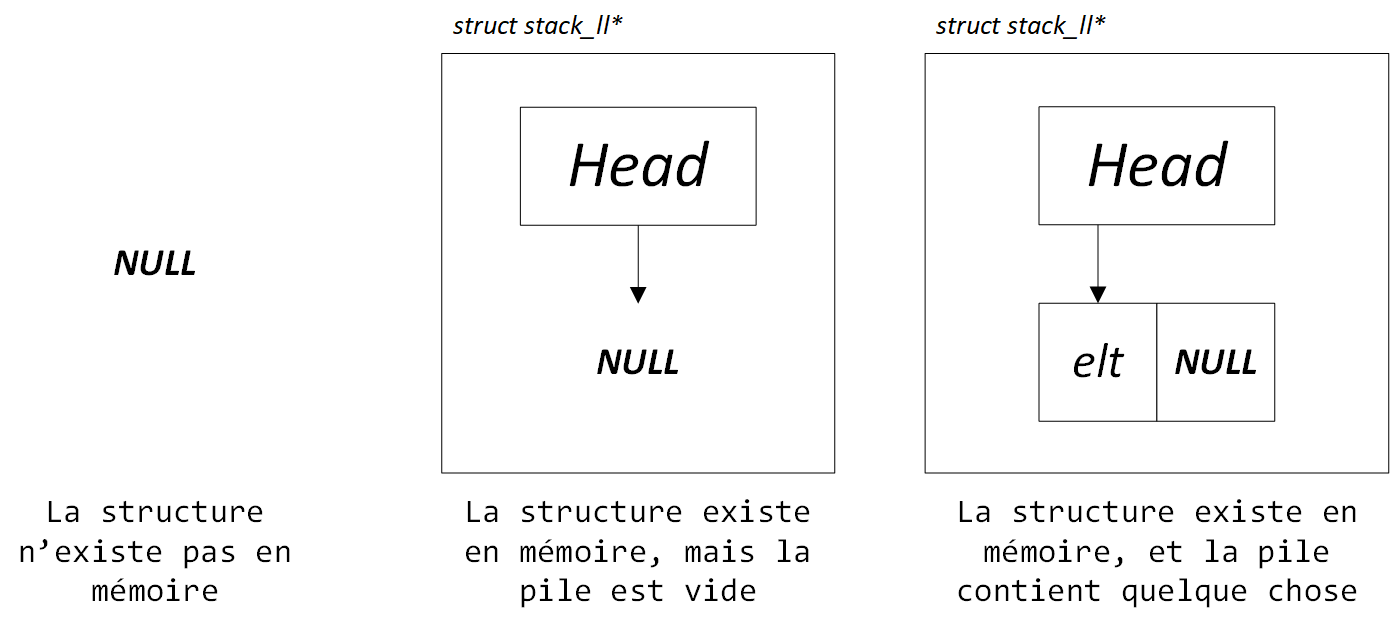
\includegraphics[scale=0.85]{Cours/Piles_Implementation_LL.png}
%\end{center}

\bigskip
%\newpage

\noindent Vous devez implémenter les fonctions suivantes :

\bigskip
%\medskip

\lstset{language=C}
%\begin{lstlisting}[frame=single,title={Liste des fonctions pour une pile avec liste chaînée}]
\begin{lstlisting}[frame=single]
list_linked *add_elt_list_linked(list_linked *list,
                                 int elt,
                                 int pos);
list_linked *del_elt_list_linked(list_linked *list,
                                 int pos);

int length_list_linked(list_linked *list);
int is_empty_list_linked(list_linked *list);

void print_list_linked(list_linked *list);

int search_elt_list_linked(list_linked *list,
                           int elt);
int get_elt_list_linked(list_linked *list,
                        int pos);

int clear_list_linked(list_linked *list);
\end{lstlisting}


\clearpage


\subsubsection*{\TTBF{list\_linked *add\_elt\_list\_linked(list\_linked *list, int elt, int pos)}}

\noindent Cette fonction ajoute un élément à la position indiquée de la liste chaînée donnée en paramètre.

\smallskip

\noindent Si la liste est vide, il faut y créer un premier élément qui sera considéré comme en position $ 1 $.

\noindent Si l'élément \textit{elt} donné en paramètre est inférieur à $ 1 $, la fonction doit renvoyer un pointeur \TTBF{NULL} sans rien modifier dans la liste.

\noindent Si la position n'existe pas (c'est-à-dire si elle est inférieure strictement à $ 1 $ ou supérieure strictement à la taille de la liste + 1), la fonction doit renvoyer un pointeur \TTBF{NULL} sans rien modifier dans la liste.
Si un élément se trouve déjà en position \textit{pos}, il faut décaler cet élément un cran vers la fin (de na position \textit{n} à la position \textit{n+1}), puis, on ajoute le nouvel élément à la position donnée en paramètre.
%Si la position \textit{pos} est négative ou à $ 0 $, il faut ajouter l'élément \textit{elt} en début de liste à la position $ 0 $ (c'est-à-dire qu'il deviendra le premier élément).
%Si la position \textit{pos} est supérieure ou égale à la taille de la liste, il faut ajouter l'élément en fin de liste (c'est-à-dire qu'il deviendra le dernier élément).

\smallskip

\noindent La fonction doit retourner un pointeur vers la tête de liste, ou vers l'éventuelle nouvelle tête de liste si celle-ci a été modifiée.
%
En cas d'erreur (pas assez de mémoire), cette fonction doit renvoyer un pointeur \TTBF{NULL}.
%\textit{Vous n'avez pas à allouer d'espace pour stocker l'élément \TTBF{elt} : c'est à l'utilisateur de votre bibliothèque de le faire.}

%\smallskip
%
%\noindent Si plusieurs cas d'erreur se produisent simultanément, leur gestion doit se faire dans cet ordre précisément : le test de la valeur de l'élément en premier, puis le test de la position, puis en dernier la mémoire insuffisante.

\bigskip


\subsubsection*{\TTBF{list\_linked *del\_elt\_list\_linked(list\_linked *list, int pos)}}

\noindent Cette fonction supprime l'élément à la position indiquée de la liste chaînée donnée en paramètre.

\smallskip

\noindent Si la liste donnée en paramètre est vide, cette fonction doit renvoyer un pointeur \TTBF{NULL}.
%Si la position \textit{pos} est négative ou à $ 0 $, il faut supprimer l'élément en position $ 0 $, c'est-à-dire le premier de la liste.
%Si la position \textit{pos} est supérieure ou égale à la taille de la liste, il faut supprimer le dernier élément de la liste.
Si la position n'existe pas (c'est-à-dire si elle est inférieure strictement à $ 1 $ ou supérieure strictement à la taille de la liste), la fonction doit renvoyer un pointeur \TTBF{NULL} sans rien modifier dans la liste.

\smallskip

\noindent La fonction doit retourner un pointeur vers la tête de liste, ou vers l'éventuelle nouvelle tête de liste si celle-ci a été modifiée.

%\smallskip
%
%\noindent Si plusieurs cas d'erreur se produisent simultanément, leur gestion doit se faire dans cet ordre précisément : le test de la liste vide en premier, puis en dernier le test de la position.

\bigskip


\subsubsection*{\TTBF{int length\_list\_linked(list\_linked *list)}}

\noindent Cette fonction renvoie la taille de la liste donnée en paramètre, c'est-à-dire le nombre d'éléments présents dans la liste.

\smallskip

\noindent Si la liste donnée en paramètre est \TTBF{NULL}, la fonction doit renvoyer $ 0 $.

\bigskip


\subsubsection*{\TTBF{int is\_empty\_list\_linked(list\_linked *list)}}

\noindent Cette fonction teste si la liste est vide ou non.

\smallskip

\noindent Si la liste est vide, c'est-à-dire si le pointeur est \TTBF{NULL}, il faut renvoyer $ 1 $ (l'équivalent de \textit{true} en C), sinon, si la liste n'est pas vide, il faut renvoyer $ 0 $ (l'équivalent de \textit{faux} en C).

\bigskip


\subsubsection*{\TTBF{void print\_list\_linked(list\_linked *list)}}

\noindent Cette procédure affiche les éléments de la liste.
Chaque élément doit être suivi d'un retour à la ligne.

\smallskip

\noindent Si la liste donnée en paramètre est vide, la procédure ne fait rien.

\noindent Le format attendu est le suivant :

\bigskip

\noindent \TTBF{\textit{elt}\textbackslash{}n}

\bigskip

\noindent Ce qui donnerait cet affichage pour la liste suivante :

\begin{table}[ht!]
  \centering
  \begin{minipage}{0.45\textwidth}
    \centering

\lstset{language=sh}
\begin{lstlisting}[frame=single]
$ ./liste_ll_example1
42
21
8
24
64
$
\end{lstlisting}

  \end{minipage}
  \hfillx
  \begin{minipage}{0.45\textwidth}
    \centering

\begin{tabular}{m{1cm} C{0.5cm} C{0.5cm} C{0.5cm} C{0.5cm} C{0.5cm} }
pos & 1 & 2 & 3 & 4 & 5 \\
\end{tabular}

\begin{tabular}{m{1cm}|C{0.5cm}|C{0.5cm}|C{0.5cm}|C{0.5cm}|C{0.5cm}|}
\cline{2-6}
elt & 42 & 21 & 8 & 24 & 64 \\
\cline{2-6}
\end{tabular}

  \end{minipage}
\end{table}

\vspace*{-0.5cm}


\subsubsection*{\TTBF{int search\_elt\_list\_linked(list\_linked *list, int elt)}}

\noindent Cette fonction cherche un élément et renvoie sa position.

\smallskip

\noindent La première position démarre à la valeur $ 1 $.

\smallskip

\noindent Si la liste donnée en paramètre est \TTBF{NULL}, la fonction doit renvoyer $ -1 $.
Si l'élément n'est pas trouvé, la fonction doit renvoyer $ -2 $.

\smallskip

\noindent Si plusieurs cas d'erreur se produisent simultanément, leur gestion doit se faire dans cet ordre précisément : le test de la liste vide en premier, puis en dernier le test de l'existence de la valeur.

\bigskip


\subsubsection*{\TTBF{int get\_elt\_list\_linked(list\_linked *list, int pos)}}

\noindent Cette fonction renvoie l'élément présent à la position indiquée.

\smallskip

\noindent Si la liste donnée en paramètre est \TTBF{NULL}, la fonction doit renvoyer $ -1 $.

%\noindent Si la position n'existe pas (c'est-à-dire si elle est inférieure strictement à $ 0 $ ou supérieure ou égale à la taille de la liste), la fonction doit renvoyer $ -2 $.
\noindent Si la position n'existe pas (c'est-à-dire si elle est inférieure strictement à $ 1 $ ou supérieure strictement à la taille de la liste), la fonction doit renvoyer $ -2 $.

\smallskip

\noindent Si plusieurs cas d'erreur se produisent simultanément, leur gestion doit se faire dans cet ordre précisément : le test de la liste vide en premier, puis en dernier le test de la position.

\bigskip


\subsubsection*{\TTBF{int clear\_list\_linked(list\_linked *list)}}

\noindent Cette fonction vide la liste de tous ses éléments, puis renvoie le nombre d'éléments qui ont été supprimés.

\smallskip

\noindent Si la liste donnée en paramètre est \TTBF{NULL}, la fonction doit renvoyer $ 0 $.
